\input{../preamble.tex}

\SetDate[02/04/2026]
\reversemarginpar
\setlength{\marginparsep}{.5cm}

\begin{document}
\pagestyle{fancy}
\fancyhead[L]{Première}
\fancyhead[C]{\textbf{Évaluation blanche — Dérivation}}
\fancyhead[R]{\today}

\null\vspace{-30pt}
Consignes particulières : 
\begin{itemize}[label=$\bullet$]
	\item 
	La calculatrice est {interdite}.
	\item
	L'évaluation fait \pageref{lastpage} pages. La somme des points est \total{points}.
\end{itemize}

\marginpar{[pts]}
\hrule

%\subsection*{Automatismes}



\exe{4,difficulty=0}{
	Considérons la fonction $f$ donnée graphiquement ci-dessous.
	\begin{enumerate}
		\item 
		Quel est le signe de $f(2)$ ?
		\item 
		Quel est le signe de $f'(2)$ ?
		\item 
		Donner approximativement la valeur de $f'(1)$.
		\item
		La tangente à $\C_f$ en $x=1$ a pour équation $y=8,3-4,4x$.
		En déduire la valeur de $f'(1)$.
	\end{enumerate}

	\begin{center}
	\begin{tikzpicture}[>=stealth, scale=1]
	\begin{axis}[xmin=-1, xmax=4, ymin=-6, ymax=6, axis x line=middle, axis y line=middle, axis line style=-, grid=both, xtick distance = 1, minor tick num = 1, clip=false]
		\addplot[BLUE_E, very thick, domain=-1:4, samples=100] {(x-.05+.75)*(x-.05-1.5)*(x-.05-4)+1}  node[right] {$\C_{f}$};
		\addplot[RED_E, <->, thick, domain=.5:1.75, samples=2, xshift=.5pt, yshift=.5pt] {8.29425-4.4425*x}  node[pos=0, right] {$y = 8,3 - 4,4x$};
	\end{axis}
	\end{tikzpicture}
	\end{center}

}{exe:tangente-graphique}{
}

\exe{3,difficulty=0}{
	La courbe représentative d'un fonction $f$ est donnée ci-dessous.
	Compléter son tableau de signes.

	\begin{multicols}{2}
	\begin{tikzpicture}[>=stealth, scale=1]
	\begin{axis}[xmin=-.1, xmax=3, ymin=-3, ymax=4, axis x line=middle, axis y line=middle, axis line style=-, grid=both, xtick distance = 1, minor tick num = 1]
		
		% (f')
		%\addplot[myr, very thick, domain =-2:3, samples=50] {(x+1)*x*(x-2)+.5}  node[pos = .77, right=2pt] {$\C_{f'}$};
		\addplot[RED_E, very thick, domain=0:3, samples=50] {sin(180*x)+(x-1)^2-1}  node[pos = 1, right] {$\C_{f}$};
	\end{axis}
	\end{tikzpicture}
	\hfill
	\vfill
	\begin{tikzpicture}
		\tkzTabInit
		 %[lgt=3,espcl=1.5]
	       		{$x$ / 1 , Signe de $f(x)$ / 2}
	       		{,,}
	\end{tikzpicture}
	\vfill\null
	\end{multicols}
}{exe:lecture-graphique}{
}




%\subsection*{Exercice}


\exe{3}{
	Donner la fonction dérivée de chaque fonction suivante.
	\begin{multicols}{2}
	\begin{enumerate}
		\item $f(x) = x^3 + 2x^2 + 6x + 10$
		\item $g(x) = -x^2 + 7x - 1$
	\end{enumerate}
	\end{multicols}
}{exe:derivation}{
}

\exe{4}{
	Développer et réduire chaque expression suivante.
	\begin{multicols}{3}
	\begin{enumerate}
		\item $f(x) = (x+1)(x+2)$
		\item $g(x) = (2x-3)(x+2)$
		\item $h(x) = 3(x+1)(x-4)$
	\end{enumerate}
	\end{multicols}
}{exe:derivation}{
}

\exe{6,difficulty=1}{
	Nous étudions une fonction $f$ pour des antécédents $x$ situés entre $-3$ et $2$.
	
	Nous disposons des informations suivantes sur $f$.
	\begin{multicols}{2}
	\begin{itemize}
		\item
		Sa dérivée est 
			$ f'(x) = (2x+3)(x-1). $
		\item
		L'image de $-3$ est $f(-3) \approx -4,6$
		\item
		L'image de $-1,5$ est $f(-1,5) \approx 3,2$
		\item
		L'image de 1 est $f(1) = -2$
		\item
		L'image de 2 est $f(2) \approx 1,2$
	\end{itemize}
	\end{multicols}
	\begin{enumerate}
		\item Remplir le tableau de signes et de variations de la figure \ref{fig:var-signe}.
		\item Compléter les variations avec les images connues de $f$.
		\item En déduire le maximum et le minimum de $f$ sur le domaine d'étude.
		\item Utiliser le tableau de variations pour esquisser $\C_f$ dans le repère figure \ref{fig:Cf}.
	\end{enumerate}
}{exe:variations-d3}{
}


\begin{figure}[h]
	\centering	
	\begin{tikzpicture}
		\tkzTabInit
		 %[lgt=3,espcl=1.5]
	       		{$x$ / 1 , Signe de $2x+3$ / 1, Signe de $x-1$ / 1, Signe de $f'(x)$ / 1, Variation de $f(x)$ / 2}
	       		{$-3$,,,,2}
	\end{tikzpicture}
	\caption{Tableau de variations de $f$ et de signes de $f'$.}
	\label{fig:var-signe}
\end{figure}

\begin{figure}[h]
	\centering
	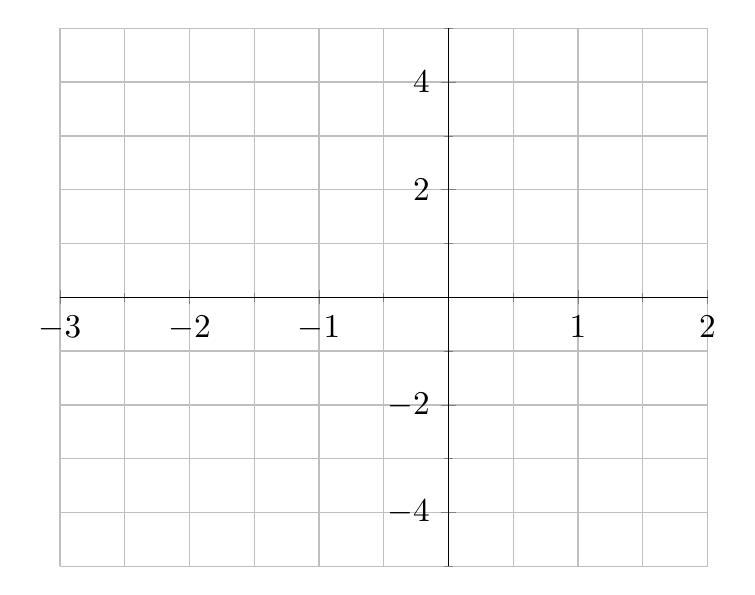
\begin{tikzpicture}[scale=1.2]
	\begin{axis}[
		xmin = -3, xmax=2,
		ymin=-5, ymax=5,
		axis x line=middle, 
		axis y line=middle, 
		axis line style=-,
		grid = both, % xlabel={$x$}, ylabel={$f(x)$},
		minor tick num = 1,
	%xtick = {0, 0.2, ..., 1.4},
	%ytick = {-1, -0.5, 0, .5, 1.5},
	]
	\addplot[domain=-3:2, transparent, thick, samples=100] {2*x^3/3 + x^2/2 - 3*x-1/6} node[right]{$\C_f$};
	\end{axis}
	\end{tikzpicture}
	\caption{Graphe approximatif de $\C_f$.}
	\label{fig:Cf}
\end{figure}


%%%%%%%%%%%%

\label{lastpage}
\newpage
\fancyhead[C]{\textbf{Solutions}}
\shipoutAnswer

\end{document}
